% chktex-file 1
% chktex-file 29

\FILENAME

\section{Intorduction to Docker}
\label{Docker}
\index{Docker}

Docker is the company driving the container movement and the only
container platform provider to address every application across the
hybrid cloud. Today's businesses are under pressure to digitally
transform but are constrained by existing applications and
infrastructure while rationalizing an increasingly diverse portfolio
of clouds, datacenters and application architectures. Docker enables
true independence between applications and infrastructure and
developers and IT ops to unlock their potential and creates a model
for better collaboration and innovation. An overview of docker is
provided at

\URL{https://docs.docker.com/engine/docker-overview/}

\begin{figure}[htbp]
\centering
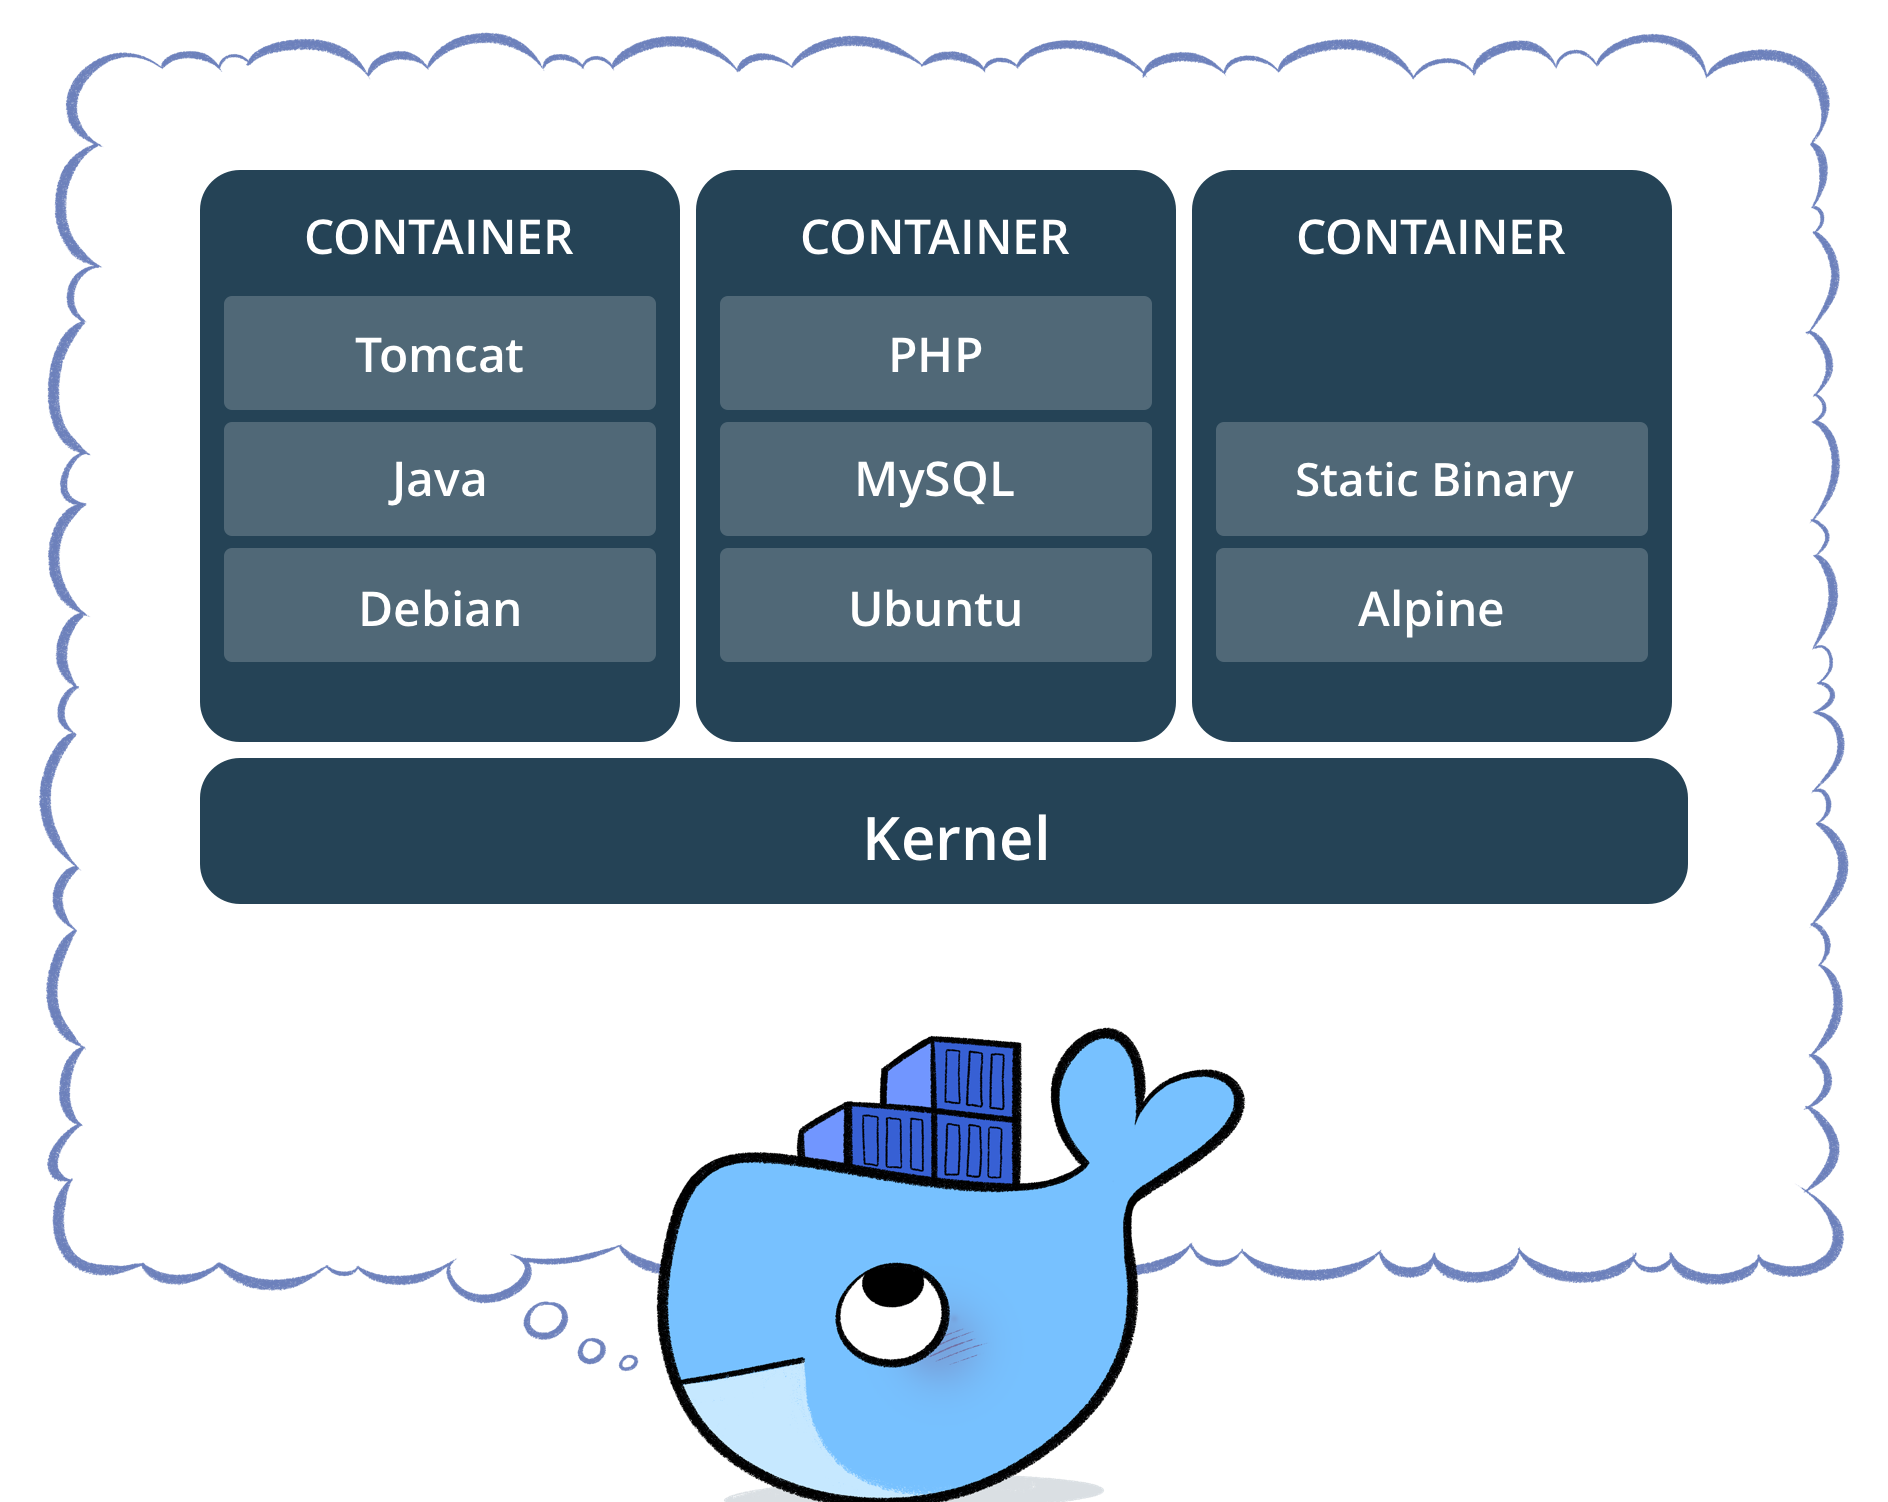
\includegraphics[width=0.7\textwidth]{docker-container.png}
\caption{Docker Containers}
\end{figure}

Image Source
\url{https://www.docker.com/sites/default/files/Package\%20software\%40x2.png}


\section{Docker Survey}

In 2016 Docker Inc.\ surveyed over 500 Docker developers and operations
experts in various phases of deploying container-based
technologies. The result is available in the \textit{The Docker Survey
  2016}.

\URL{https://www.docker.com/survey-2016}

\begin{figure}[htb]
\centering
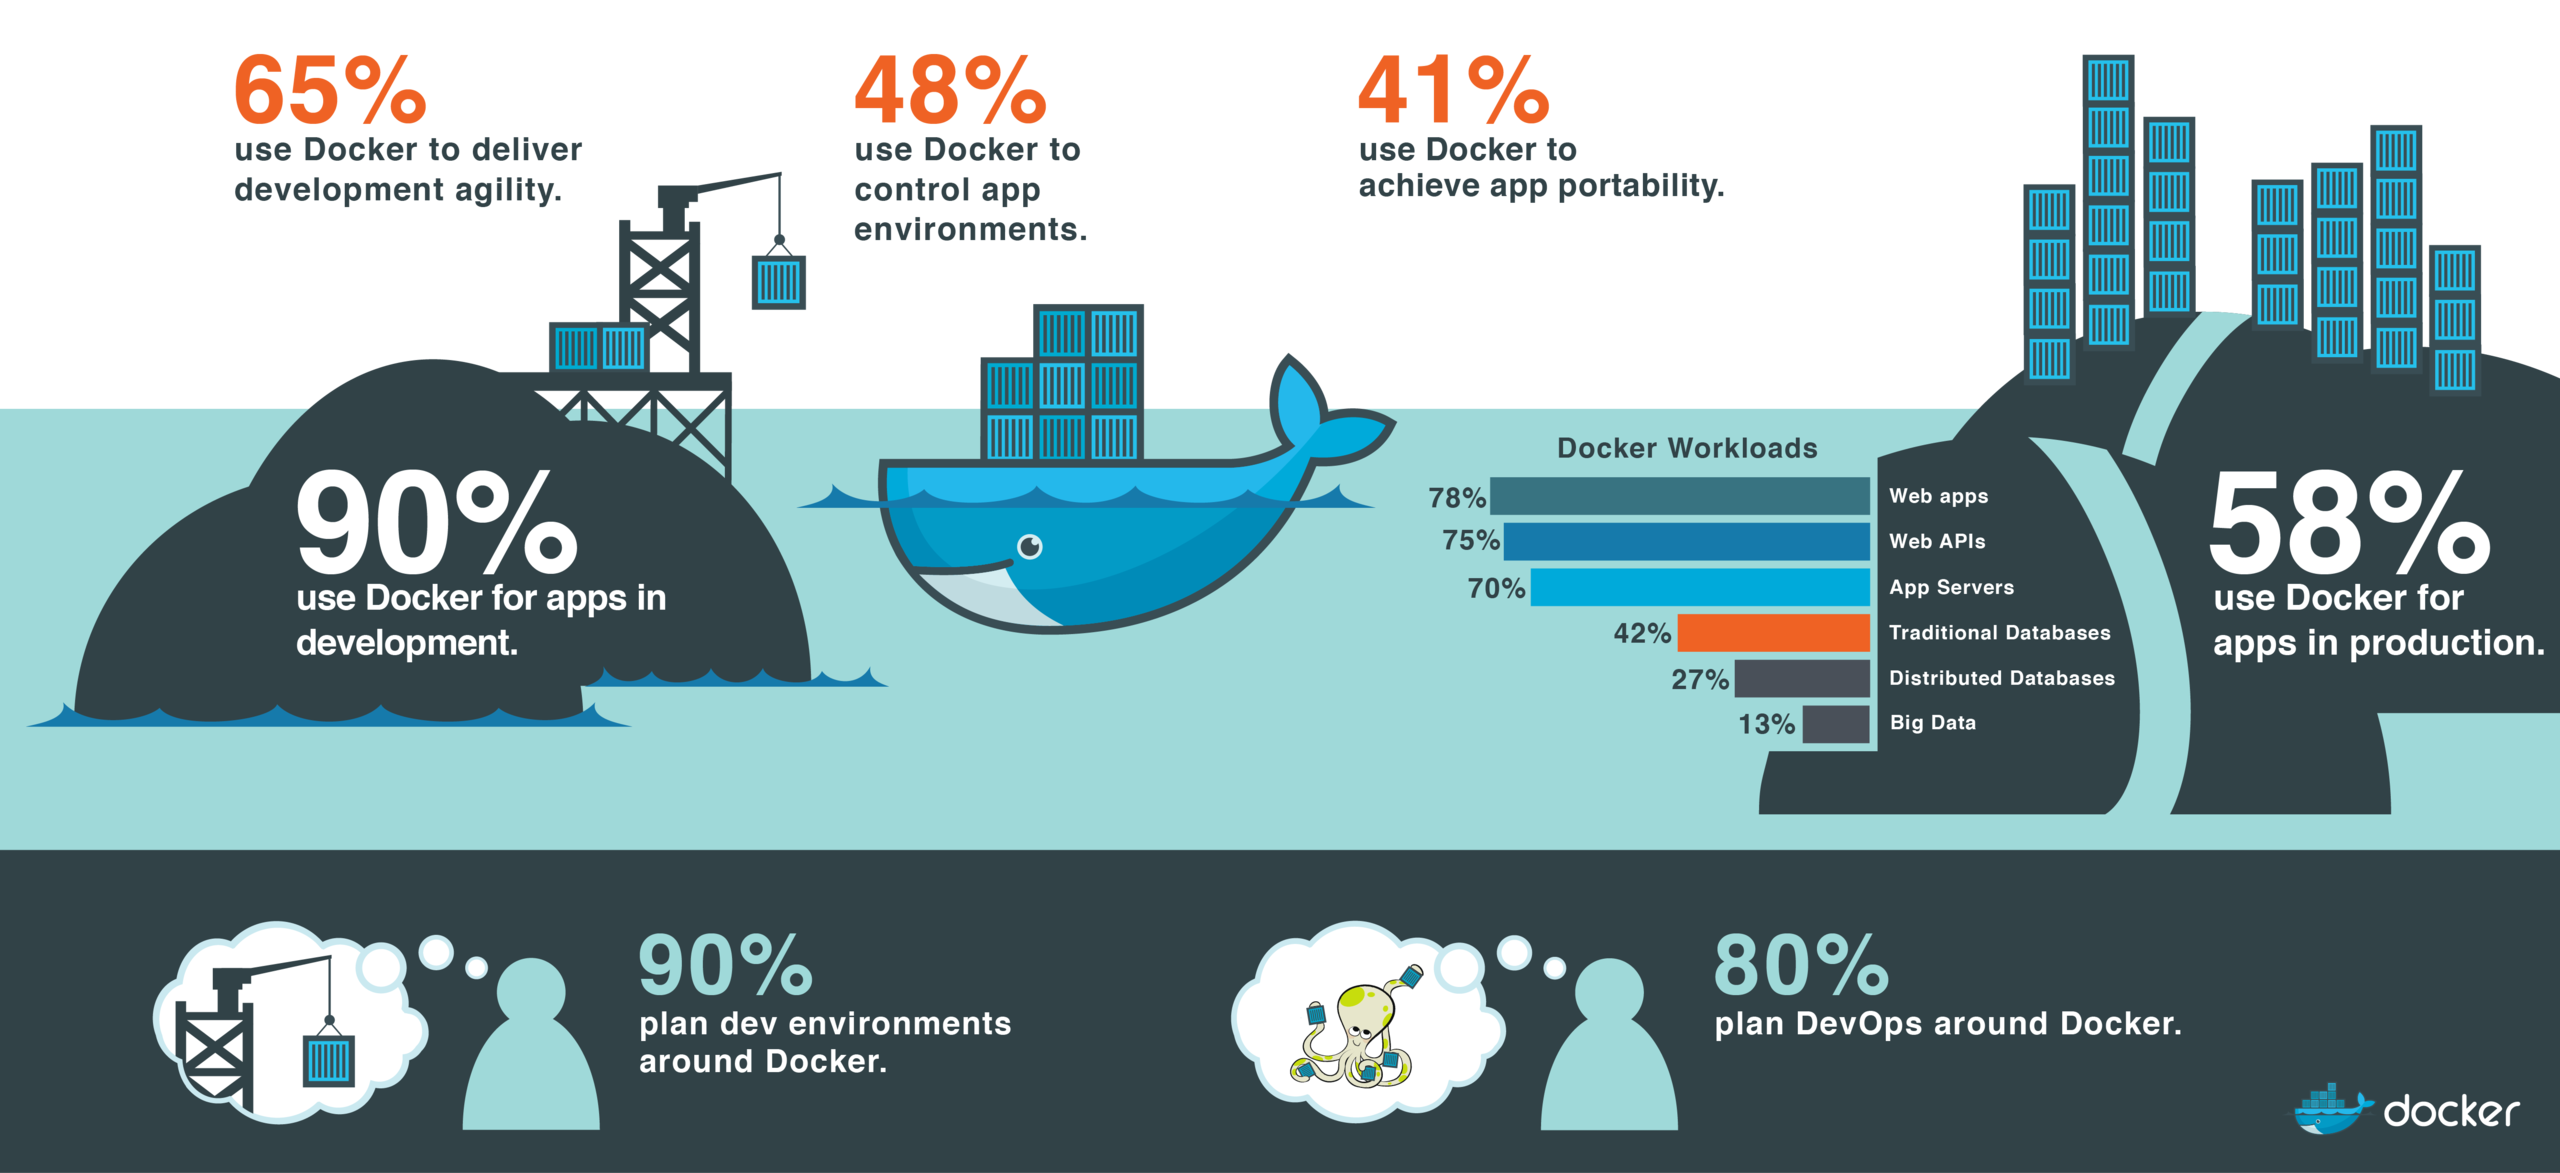
\includegraphics[width=1.0\textwidth]{images/docker-survey.png}
\caption{Docker Survey Results 2016
}
\end{figure}


\begin{figure}[htb]
\centering
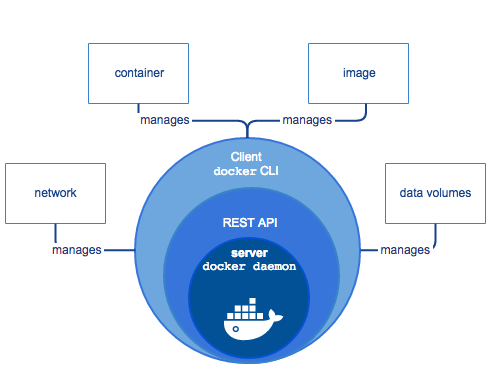
\includegraphics[width=0.5\textwidth]{images/engine-components-flow.png}
\caption{ Docker Engine Component Flow }
\end{figure}

\begin{figure}[htb]
\centering
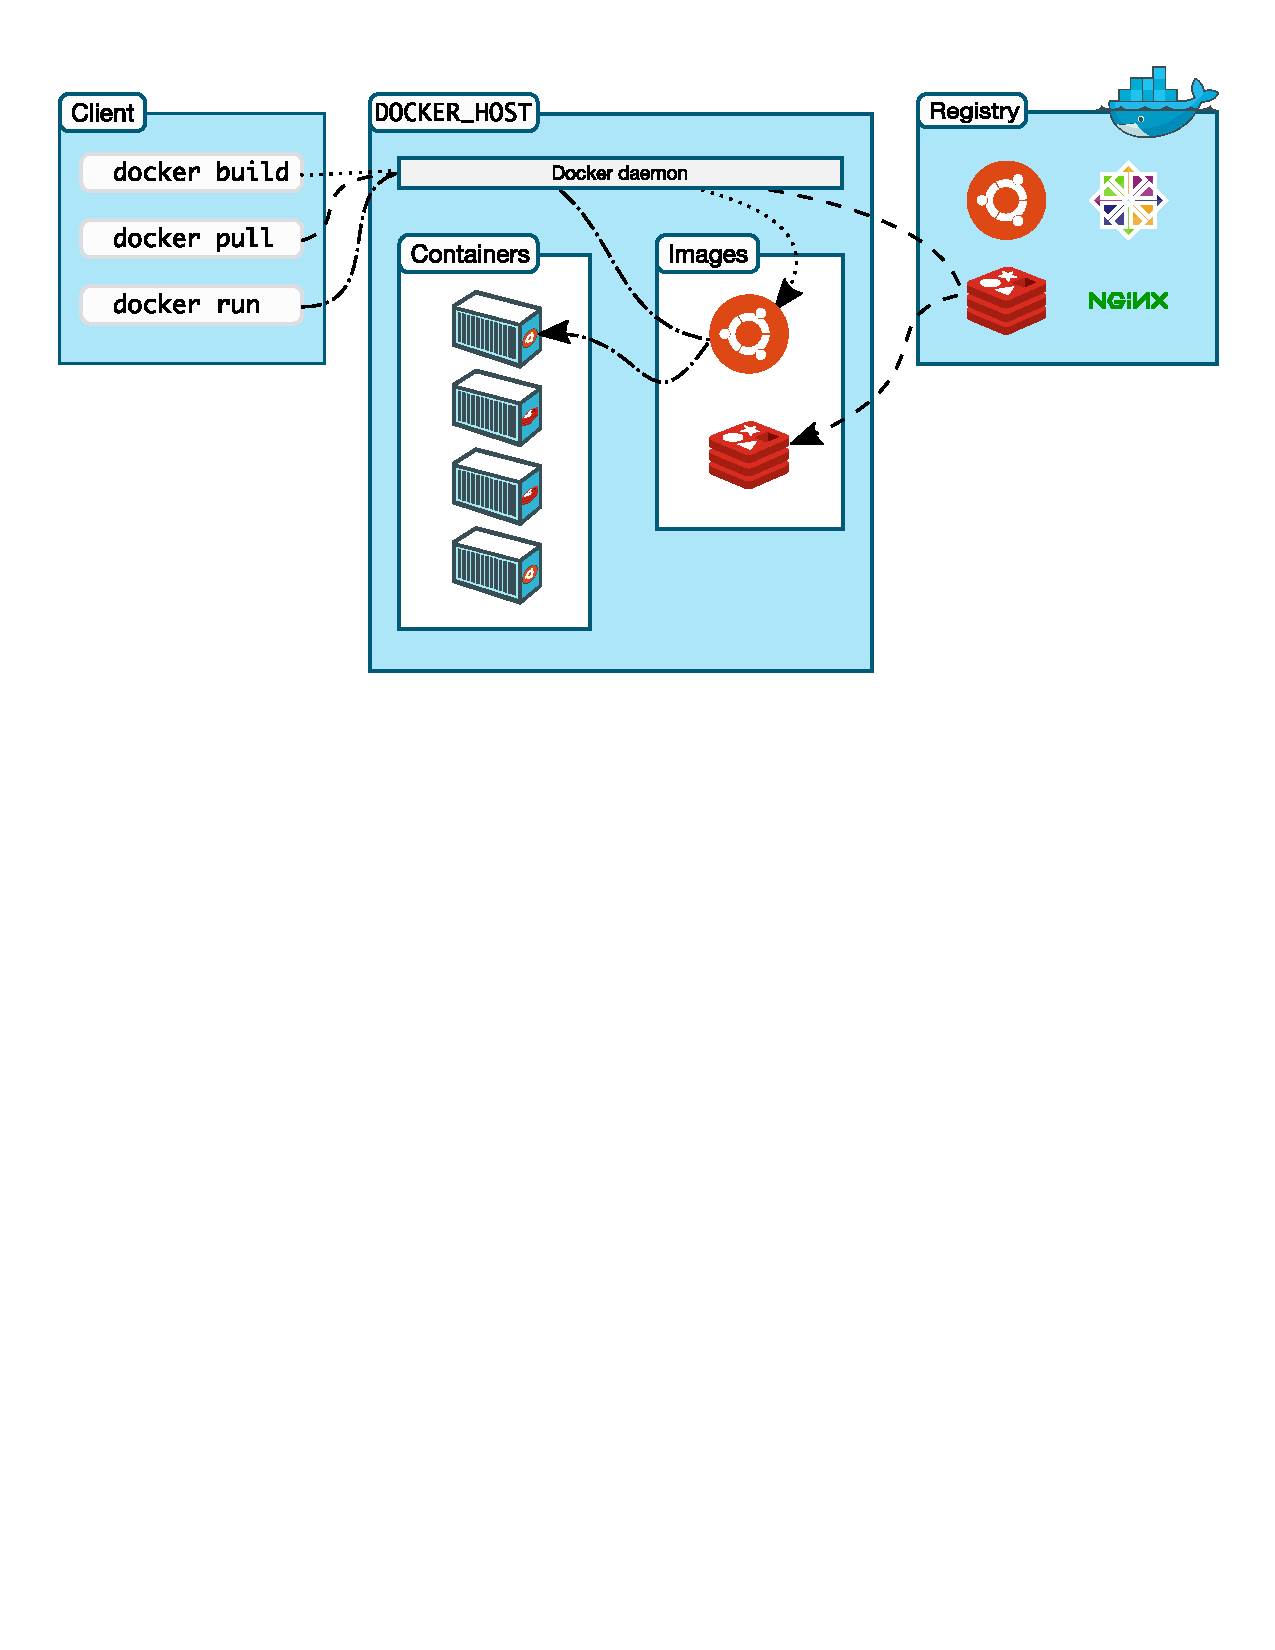
\includegraphics[width=1.0\textwidth]{images/docker-architecture.pdf}
\caption{ Docker Architecture }
\end{figure}

